\documentclass{IEEEtran}
\usepackage[utf8]{inputenc}
\usepackage{listings}
\usepackage{cite}
\usepackage{amsmath,amssymb,amsfonts}
\usepackage{algorithmic}
\usepackage{graphicx}
\usepackage{textcomp}
\usepackage{xcolor}
\usepackage{color}
\usepackage{url}
\usepackage{caption}
\definecolor{dkgreen}{rgb}{0,0.6,0}
\definecolor{gray}{rgb}{0.5,0.5,0.5}
\definecolor{mauve}{rgb}{0.58,0,0.82}
\lstset{%
    aboveskip=3mm, belowskip=3mm,
    showstringspaces=false,
    columns=flexible,
    basicstyle={\small\ttfamily},
    numbers=none,
    numberstyle=\tiny\color{red},
    keywordstyle=\color{blue},
    commentstyle=\color{dkgreen},
    stringstyle=\color{mauve},
    breaklines=true,
    breakatwhitespace=true,
    tabsize=3
}

\newcommand{\code}[1]{\texttt{#1}}
\newcommand{\val}[1]{#1_{\text{val}}}
\newcommand{\est}[1]{#1_{\text{est}}}

\def\BibTeX{{\rm B\kern-.05em{\sc i\kern-.025em b}\kern-.08em
    T\kern-.1667em\lower.7ex\hbox{E}\kern-.125emX}}
\begin{document}
\title{Lab1 --- Fundamental Signal Processing}

\maketitle

\section{Introduction}
This report describes a laboratory performed at Linköping university as an
assignment in a course in digital signal processing. In the context of
digital signal processing, it is possible to create a model of a given
signal that can be used later on to recreate the original signal to some
extent. These models can usually be described with a number of parameters
that is much lower that the number of samples in the actual signal. Because
the recreated signal would just be an approximation of the original signal
it is important to analyze how well the model describes the signal as well
as what can be done to improve the model. The purpose of the laboratory was
to experiment with how this might be done in practice.

The laboratory consisted of three parts, each with different tasks and
goals.

The first assignment was to model the sound of a person whistling and the
try to recreate the sound from the model. Focus lay on analyzing the purity
of the recreated signal.

The goal of the second part was to create models for the sound of spoken
vowels and then recreate the sounds. The main task here was to estimate
the model order needed for each sound and the validate the resulting
sounds against the original sounds.

The last part of the laboratory consisted of recording and modeling of
spoken language in a similar way as it would be done in GSM communication.
The focus of this task lay on implementing the modeling method and analyze
the results.

\section{Assignment 1 --- Whistle}
Asignment 1 consisted of recording the sound of a person whistling and then
modeling it.

\subsection{Theory}
\label{sec:whistletheory}
The sound of whistling is relatively simple and pure sound that resembles
a sine wave. Therefore it is expected to be possible to model this sound
with a simple model with only a small number of parameters. Such a model
could be for example an auto-regressive model of order 2. An AR(2) model
can be described mathematically as follows,

\begin{equation}
  \label{1:ar2}
  y(t) + a_1 y(t-1) + a_2 y(t-2) = e(t) \quad .
\end{equation}

In Equation \ref{1:ar2}, $y$ is the signal generated by the model, $e$ is
simply white noise and $a_1, a_2$ are the parameters that describe the
model. This means that the signal can be generated from the previous two
generated sample and white noise:

\begin{equation}
  \label{1:ar2y}
  y(t) = e(t) - a_1 y(t-1) - a_2 y(t-2)\quad .
\end{equation}

The parameters $a_1$ and $a_2$ are describing the behaviour of the system
while the purpose of $e$ is to input energy in to the system. Any signal
$e$ that has a constant power spectrum can be used to generate the desired
signal as described by \textit{Wold's theorem}\cite{signalproc}. In this
case though, the signal of the whistling sound resembles white noise more
than the other alternatives. Therefore, white noise should be used to
recreate the signal as it is expected to give the best results.

It is expected that the generated signal from the model is not exactly
equal to the original one because the model is described with only a small
number of parameters. Thus, the recreated signal is expected to be just an
approximation of the original one. For this reason it is of interest to
try to find the model parameters in such a way that generates a signal
that is as close as possible to the desired one. Given the original signal
$s$ and the generated signal $y$, it is desired to find the set of
parameters $\theta$ so that the loss function
\begin{equation}
  \label{1:loss}
  V(\theta)  = \frac{1}{N}\sum_{t=1}^{N}(s(t) - y(t; \theta))^2
\end{equation}
to be as small as possible. For example, in the case of Equation \ref{1:ar2},
$\theta$ would consist of the parameters $a_1$ and $a_2$. By defining
the regression vector
\begin{equation}
  \phi^T(t) = (y(t-1), y(t-2), ... , y(t-N)) \quad ,
\end{equation}
Equation \ref{1:ar2y} can be rewritten as
\begin{equation}
  y(t) = \phi^T(t)\cdot\theta + e(t) \quad .
\end{equation}

In these equations $e(t)$ is considered to be white noise, so when
generating a signal from the model it it impossible to know beforehand
what values $e(t)$ will take. Therefore for the purpose of estimating
the model parameters $e(t)$ can be set to its mean value which in this
case is $0$. Therefore
\begin{equation}
  \label{1:esty}
  y(t) = \phi^T(t)\cdot\theta \quad .
\end{equation}

By defining the $N\times1$ vector $Y_N$ and the $N\times n$ vector
$\Phi_N$ as following,

\begin{equation}
  Y_N =
  \begin{pmatrix}
    y(1) \\ y(2) \\ \vdots \\ y(N)
  \end{pmatrix}
  \quad
  \textnormal{and}
  \quad
  \Phi_N =
  \begin{pmatrix}
    \phi^T(1) \\ \phi^T(2) \\ \vdots \\ \phi^T(N)
  \end{pmatrix}
  \quad ,
\end{equation}
Equation \ref{1:esty} can be written in vector notation as
\begin{equation}
  Y_N = \Phi_N\theta \quad .
\end{equation}

According to \cite{signalproc} this equation can be treated as a least
squares problem and be solved through the following system of normal
equations,

\begin{equation}
  \Phi_N^T\Phi_N\theta = \Phi_N^T Y_N \quad ,
\end{equation}

where the solution is given by

\begin{equation}
  \hat{\theta}_N = \left( \frac{1}{N}\Phi_N^T\Phi_N \right)^{-1}
                   \left( \frac{1}{N}\Phi_N^T Y_N \right)
  \quad .
\end{equation}

The solution $\hat{\theta}_N$ is the desired set of model parameters
that minimizes the loss function defined in \ref{1:loss} for a signal
of length $N$. These can be later used to generate a signal that
resembles sound of whistling.

There are multiple ways to check the purity of the generated signal which
means analysing how close to a pure whistle the resulting signal is.

Since it is expected that the signal should have most of its energy
concentrated around a certain frequency, one way to check its purity
is to look at its harmonic distortion. This measure is defined as

\begin{equation}
  \label{1:hdist}
  1 - \frac{E_{\textnormal{dom. freq.}}}{E_{\textnormal{tot.}}}\quad .
\end{equation}
$E_{\textnormal{dom. freq.}}$ is in this case the energy contained in
a small frequency band centered around the signal's dominant frequency
and $E_{\textnormal{tot.}}$ is the signal's total energy. It is desired
that most of the signal's energy is concentrated around its dominant
frequency so a smaller measure of harmonic distortion means that the
signal is more pure.

Another way to measure the purity of the signal is to look at the poles
of the estimated model. The closer these poles are to the unit circle
the more pure the signal is.

\subsection{Method}
\label{sub:whistlemethod}
The first step of the laboratory was to record the sound of a person
whistling. This was done using the program \textit{Audacity}
\cite{audacity} at a sampling frequency of 8000 Hz. The recording was then
cut to a length of 2 seconds that were chosen where the quality of the
audio was best in the signal. Figure \ref{1:whistle_orig} shows a plot
of the original recording of the whistle in the time domain.

\begin{figure}[h]
  \centering
  \captionsetup{justification=centering}

  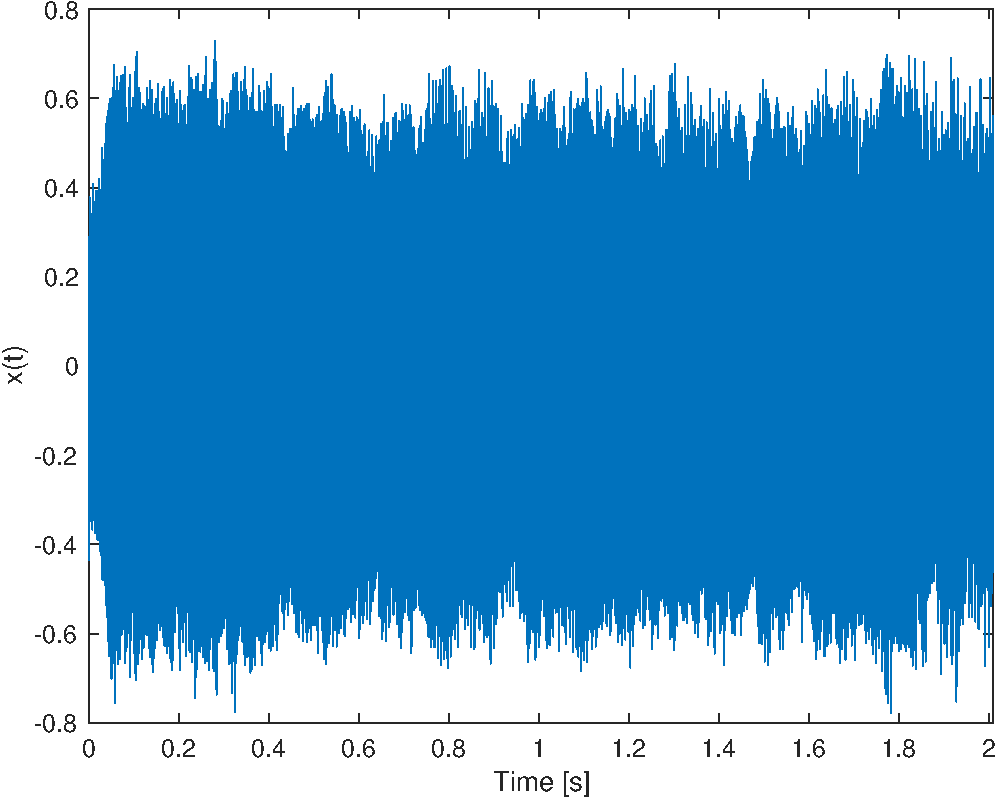
\includegraphics[width=0.8\columnwidth]{pictures/whistle_orig.pdf}
  \caption{Original whistle recording}
  \label{1:whistle_orig}

\end{figure}

The next step was to compute the signal's fourier transform and to
inspect its frequency spectrum. This spectrum is shown in Figure
\ref{1:whistle_fft}.

\begin{figure}[h]
  \centering
  \captionsetup{justification=centering}

  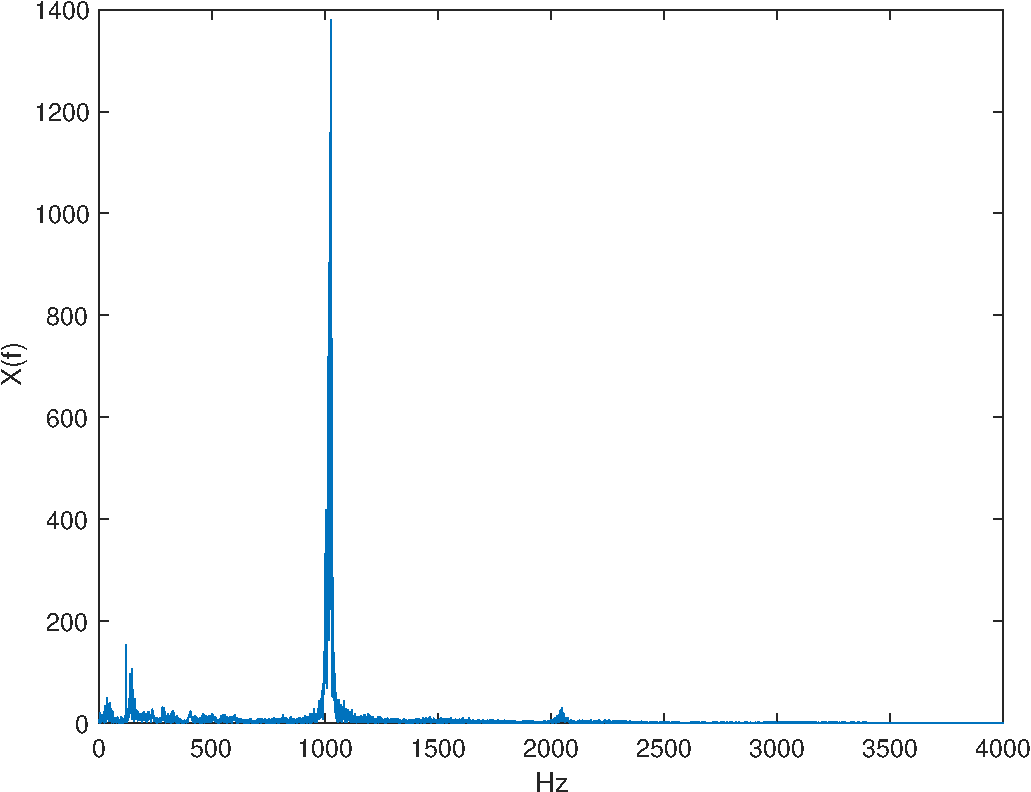
\includegraphics[width=0.8\columnwidth]{pictures/whistle_fft.pdf}
  \caption{Fourier transform of the whistle signal}
  \label{1:whistle_fft}

\end{figure}

By inspecting the plot the dominant frequency of the whistle could be
identified as approximately 1025 Hz. It can be seen in the graph that
most of the signal's energy is concentrated around this frequency as
expected. It can also be seen that there are some other unwanted
frequency components further away from the dominant frequency.

\begin{figure}[h]
  \centering
  \captionsetup{justification=centering}

  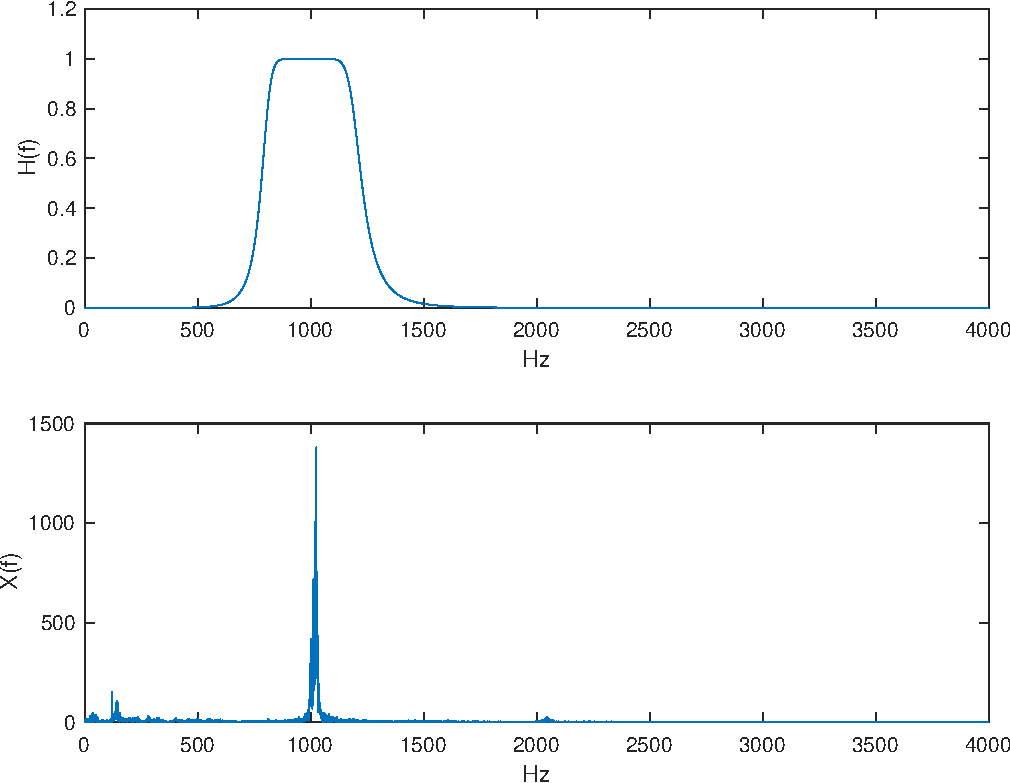
\includegraphics[width=0.8\columnwidth]{pictures/whistle_filter.pdf}
  \caption{Frequency spectrum of the butterworth filter and the original
  whistle signal}
  \label{1:whistle_filter}
\end{figure}

These components were removed by filtering the signal with a butterworth
filter of degree 5 with the pass band between 800 Hz and 1200 Hz. The
filtering was done with the \code{filtfilt} function in MATLAB which filters
the signal without altering its phase spectrum. The frequency spectrum
of the filter is shown above the original's signal spectrum in Figure
\ref{1:whistle_filter}. The frequency of the filtered signal is shown
in Figure \ref{1:whistle_clean} where it can be seen that the other
frequency components have been removed.

\begin{figure}[h]
  \centering
  \captionsetup{justification=centering}

  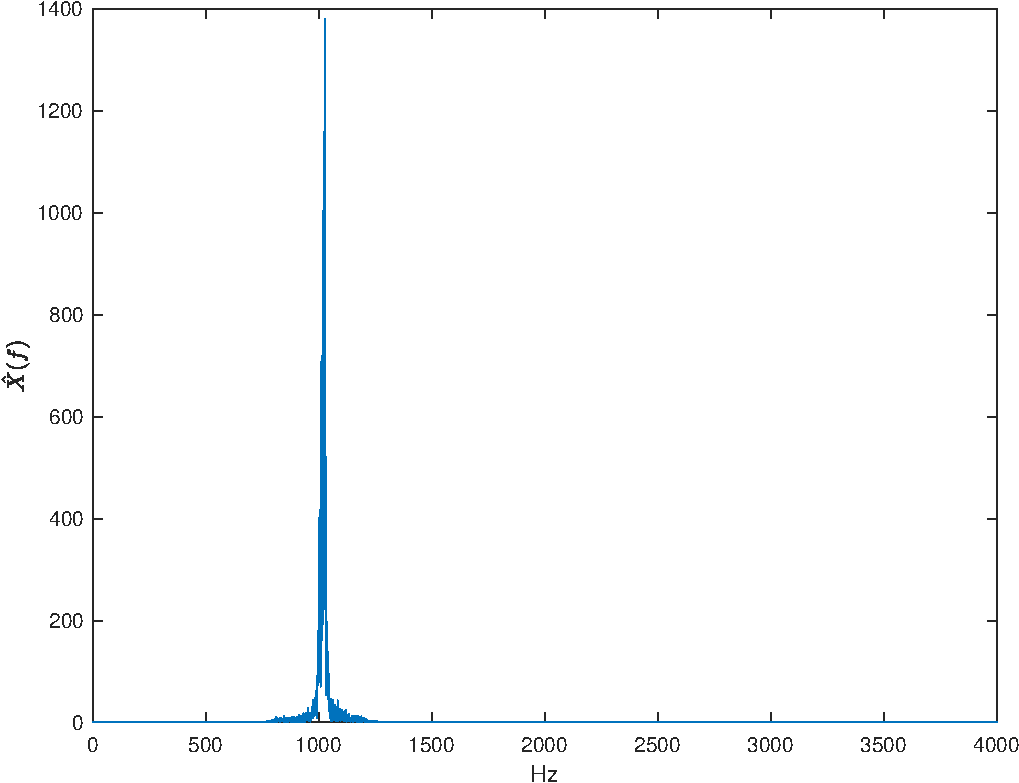
\includegraphics[width=0.8\columnwidth]{pictures/whistle_clean.pdf}
  \caption{Fourier transform of the filtered whistle signal}
  \label{1:whistle_clean}

\end{figure}

The total energy of the signal was calculated on the signal before filtering
in the time domain using the formula

\begin{equation}
  E_{tot} = \sum_k{x^2(k)} \quad
\end{equation}

and in the frequency domain using the formula

\begin{equation}
  E_{tot} = \frac{1}{N}\sum_f{X^2(f)} \quad .
\end{equation}

The energy of the dominant frequency is calculated in the same way but
using the signal after filtering, $\hat{x}(t)$, with

\begin{equation}
E_{tot} = \sum_k{\hat{x}^2(k)} \quad
\end{equation}
and
\begin{equation}
E_{tot} = \frac{1}{N}\sum_f{\hat{X}^2(f)} \quad .
\end{equation}

Now that the different measures of energy were calculated it was possible to
calculate the harmonic distortion of the original signal according to
\ref{1:hdist}. The energy in the frequency domain can also be calculated
without filtering the signal, by using the samples in the frequency spectrum
close to the dominant frequency and setting the rest to zero.

Having previously removed the unwanted frequency components, the next
step was to use the clean signal to estimate the model parameters.
This was done in accordance to the theory explained in \ref{sec:whistletheory}
by using the custom MATLAB function \code{arordercv}. The code for this
function is shown in the appendix \ref{code:arordercv}. This function also
returns the variance $\lambda_e$ the white noise should have in order to
recreate the signal properly.

After the model parameters were estimated it was time to generate a whistle
sound with the model. To do this, white noise was generated with mean $0$
and variance $\lambda_e$ using the function \code{randn}. This white noise
was input through the model as in Equation \ref{1:ar2y} and a new signal
was generated. At this point it was possible to listen to the new generated
signal and compare it to the original one. The frequency spectrum of the
simulated sound is compared to that of the original sound in Figure
\ref{1:whistle_gen_freq}.

Lastly the poles of the estimated model are computed with help of the
MATLAB function \code{tf2zp} and their distance to the unit circle was
analyzed.

The implementation of all the steps just described is shown in appendix
\ref{code:whistle}.

\begin{figure}[h]
  \centering
  \captionsetup{justification=centering}

  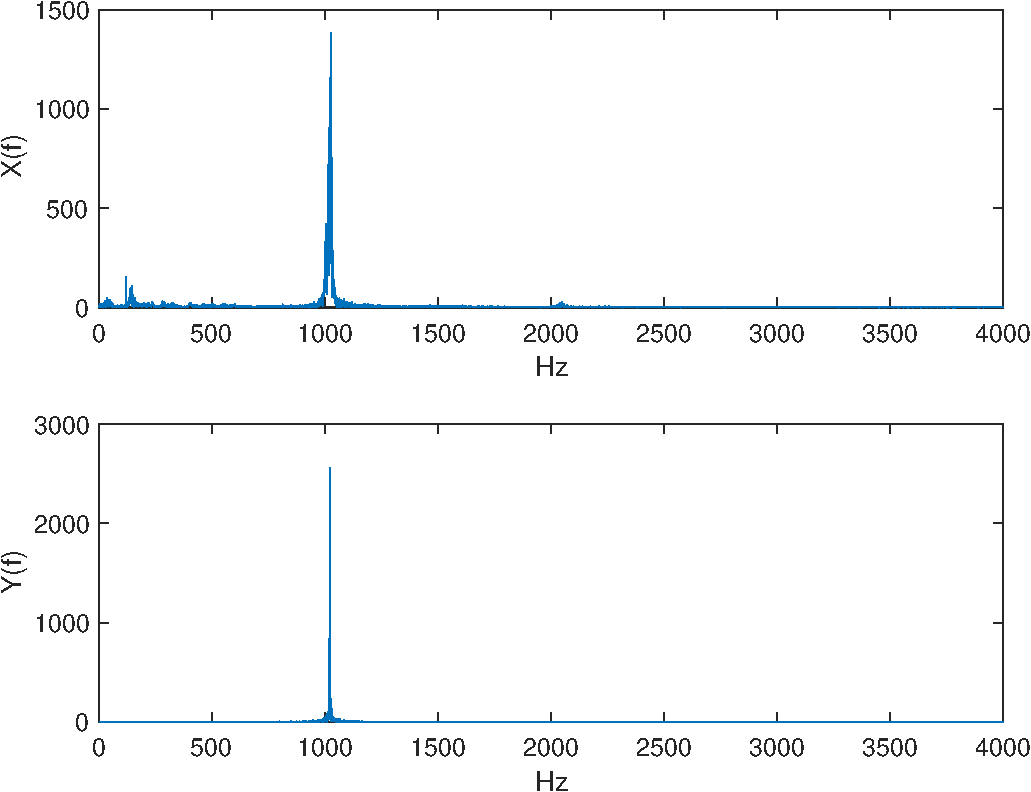
\includegraphics[width=0.8\columnwidth]{pictures/whistle_gen_freq.pdf}
  \caption{Fourier transform of the original signal and of the generated signal}
  \label{1:whistle_gen_freq}

\end{figure}

\subsection{Results}
The dominant frequency of the original whistle sound was found by inspecting
its frequency spectrum to be 1025 Hz. The same procedure showed that the
dominant frequency of the generate signal was 1019 Hz.

The total energy of the signal calculated in both the frequency domain and
the time domain was found to be $2.45\cdot10^3$. The energy of the dominant
frequency only was found to be $2.41\cdot10^3$ which is slightly lower
than the total energy.

Using these results to calculate the harmonic distortion gave a value
of $0.0157$ in both time and frequency domain.

Finally an analysis of the poles of the AR(2) showed that their distance
to the unit circle was $2.9\cdot10^{-5}$.

\subsection{Discussion}
The results show that the dominant frequency of the generated signal
differs slightly from that of the original signal. This difference can
be attributed to the fact that the estimated model only gives an
approximation of the original signal. It would require describind the
model with a higher number of parameter or possibly with another type
of model to get a better approximation. The difference in frequency
in this case is though very small and would not be noticeable
by a person when listening to the two signals.

As expected since before the experiment, most of the signal's energy
is concentrated in a small band around its dominant frequency. This
is shown by the fact that the energy around the dominant frequency is
only slightly lower than the total energy. This resulted as expected
in a low harmonic distortion measure which means that the initial
whistling recording was quite pure. This can also be concluded from
the analysis of the poles of the model which have a distance to the
unit circle that is very small.

Ultimately it should be mentioned that the generated signal resembled the
original sound remarkably well with only very hard to notice
differences. Therefore it can be concluded that an AR(2) model can
be used to model the sound of a person whistling with results that
are quite close to the original signal.

\section{Assignment 2 --- Vowel}

In this assignment, the sound of the vowels `a' and `o' were to be
modeled, using AR-models of suitable orders. The models were then
used to simulate the vowels using a suitable input signal.

\subsection{Theory}
\label{sub:voweltheory}

In this section, the theoretical background behind the vowel assignment is
explained.

\subsubsection{Model order estimation}
\label{ssub:modelorderestimation}

In order to estimate the model order, \textit{cross validation} is used.
Here, the observed data $y(t)$ is split into two
parts, the \textit{estimation data} $\est{y}(t)$ containing samples $1,
2,\ldots,N_1$, and
the \textit{validation data} $\val{y}(t)$ containing samples $N_1 + 1, N_1 + 2,
\ldots,N$,
where $N$ is the total number of observed
samples, and $N_1 = \frac{2N}{3}$.

The estimation data is used to estimate AR-models of varying orders, using
the theory explained in Section~\ref{sec:whistletheory}. We then define the
\textit{loss function} $W(n)$ as
\begin{equation}
    W(n) = V(\hat{\theta}^{(n)})
\end{equation}
where
\begin{equation}
    V(\hat{\theta}^{(n)}) = \frac{1}{\val{N}}\sum^{\val{N}}_{t=1}(\val{y}(t) -
        \val{\hat{y}}(t;\hat{\theta}^{(n)}))^2
\end{equation}
where $\hat{\theta}^{(n)}$ denotes the model parameters of the $n$:th order
AR-model generated from the estimation data. This means that $W(n)$ measures
how much the validation data differs from the predicted validation data, when
using an AR-model of order $n$. By plotting $W(n)$, a
clear picture of which model order should be used can be seen; the model order at which
increasing $n$ doesn't decrease $W(n)$ particularly much.

We denote quantity $\val{y}(t) - \val{\hat{y}}(t;\hat{\theta}^{(n)})$ as
$\epsilon(t;\hat{\theta}^{(n)})$. This quantity can equivalently be calculated
as
\begin{equation}
    \epsilon(t;\hat{\theta}^{(n)}) =
    \frac{A(q,\hat{\theta}^{(n)})}{C(q,\hat{\theta}^{(n)})}\val{y}(t)
\end{equation}
where $A(q,\hat{\theta}^{(n)})$ denotes the poles of the AR-model, and
$C(q,\hat{\theta}^{(n)})$ the zeros. This means that
$\epsilon(t;\hat{\theta}^{(n)})$ can be calculated by filtering the validation
data with the inverse of the filter created by the estimated AR-model.

\subsubsection{Model validation}
\label{ssub:modelvalidation}
The models can be validated by again using cross validation. Using residual
$\epsilon(t;\hat{\theta}^{(n)})$, a \textit{residual whiteness test} can be
performed. The residual should be approximately white if the model is accurate,
which can be tested by checking that the probability of
$\epsilon(t;\hat{\theta}^{(n)})$ changing sign from one sample to the next is
about 0.5. This is because each sample of a white process is uncorrelated with
any other sample, giving a random and unbiased sign change probability.

The whiteness of the residual can also be tested by calculating it's covariance
function $R_{\epsilon\epsilon}(k)$. The function should approximately be equal
to $\lambda\delta(t)$, where $\lambda$ is some non-zero constant.

Another way of validating the model is to simply perform a one-step-ahead
prediction of the validation data, using the estimated model from the
estimation data, and compare it with the observed validation data.

\subsubsection{Simulating}
Since a vowel is a periodic signal, it is suitable to simulate them using an
impulse train with the same period as the vowel to simulate. The amplitude
of this pulse train should be $\sqrt{\lambda T}$ where $T$ is the period and
$\lambda$ is the signal power of the vowel. $\lambda$ is estimated in conjunction with the
estimation of the AR-model.
This pulse train can be filtered with the estimated AR-model for a vowel
to simulate it.

\subsection{Method}
The vowels `a' and `o' were recorded and trimmed such that they are two seconds
long, in the same way as described in Section~\ref{sub:whistlemethod}.
Both of these recordings were split into estimation and validation parts,
as described in Section~\ref{ssub:modelorderestimation}. The function
\code{arordercv} from \cite{signalproc} implements the approach described in
that section to find the suitable model order for the `a' and `o' vowels, and is
listed in Appendix~\ref{code:arordercv}. This code plots $W(n)$ for each
vowel, and the model order at which an increase in the order doesn't
significantly decrease $W(n)$ any more is identified. A model order slightly
higher than this was selected, to have some margin. The plot of $W(n)$ for the
`a' and `o' vowels are shown in Figure \ref{fig:wna} and Figure \ref{fig:wno},
respectively.

\begin{figure}[h!]
    \centering
    \captionsetup{justification=centering}
    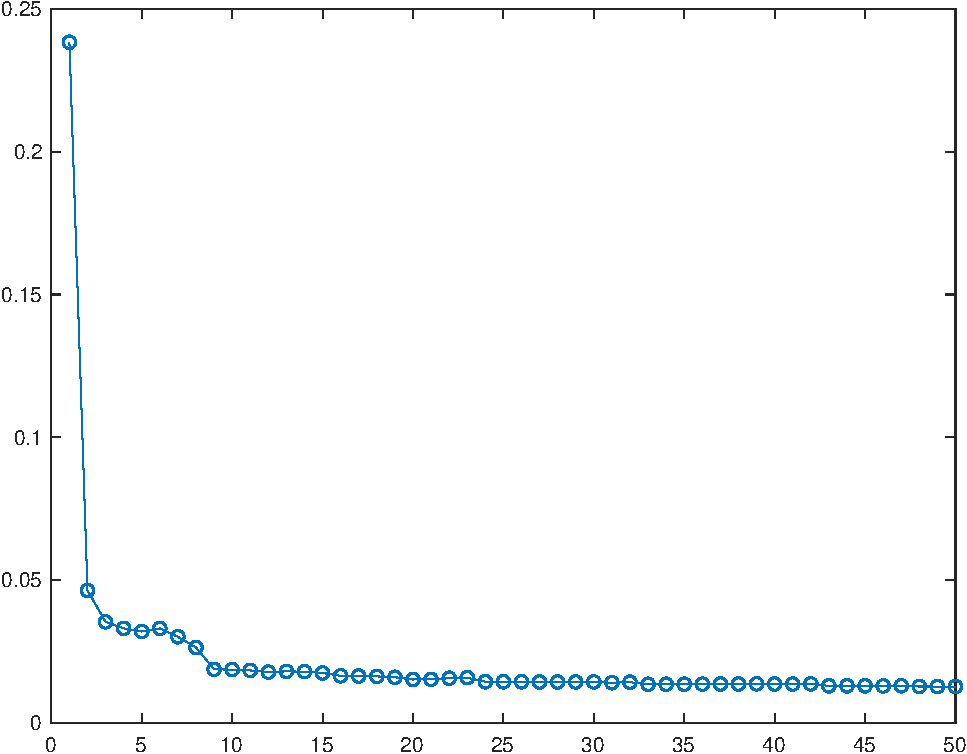
\includegraphics[width=0.8\columnwidth]{pictures/wna.pdf}
    \caption{Plot of $W(n)$ for the vowel `a'}
    \label{fig:wna}
\end{figure}

\begin{figure}[h!]
    \centering
    \captionsetup{justification=centering}
    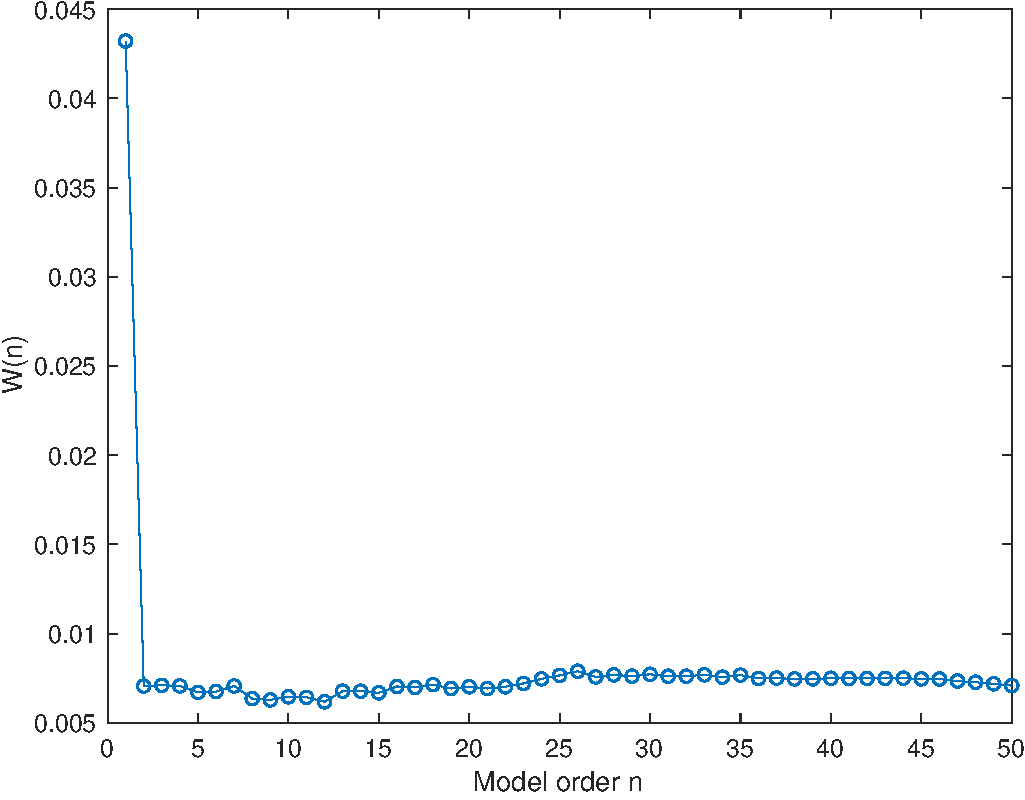
\includegraphics[width=0.8\columnwidth]{pictures/wno.pdf}
    \caption{Plot of $W(n)$ for the vowel `o'}
    \label{fig:wno}
\end{figure}

The models were then validated using residual whiteness testing and plotting of
covariance functions. The residuals were calculated according to the theory in
Section~\ref{ssub:modelvalidation}. The function \code{sign\_change\_prob}
listed in Appendix~\ref{code:signchangeprob}
measures the probability of each sample changing it's sign for the next
sample, which according to Section~\ref{ssub:modelvalidation} should be about
0.5. The covariance functions were calculated by convolving the residuals with
a time-reversed version of themselves.

The models were also validated by comparing the prediction of the validation
data for each vowel with the observed validation data. This was
done using MATLAB's \code{compare} function.

The vowels were simulated by first plotting the raw signals of each vowel, and
from the figure deduce the periods of the signals. These plots are found in
Figure \ref{fig:rawaudio}. Pulse-train signals with these
periods $T$ and amplitudes $\sqrt{\lambda T}$ were then created,
and filtered through the AR-models with appropriate
orders estimated with \code{sig2ar}, to create the simulations of each vowel.
These simulations were played back using the MATLAB command \code{sound}.

\begin{figure}[h!]
    \centering
    \captionsetup{justification=centering}
    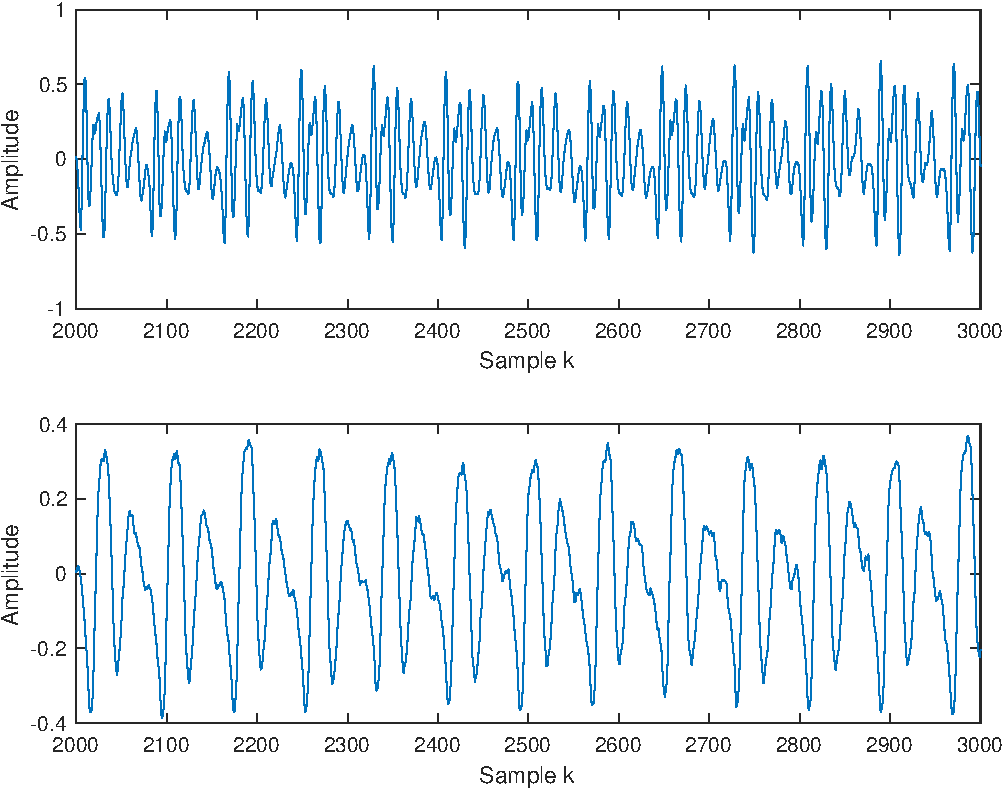
\includegraphics[width=0.8\columnwidth]{pictures/raw_o_audio.pdf}
    \caption{Plot of 1000 samples of the raw `a' audio (above) and the `o'
    (below)}
    \label{fig:rawaudio}
\end{figure}

The code performing these operations is listed in Appendix~\ref{code:vowels}.

\subsection{Results}

The appropriate model order for the `a' vowel was selected as 10, from Figure
\ref{fig:wna}, since $W(n)$ is quite flat around 10, while still giving some
margin from the steep "knee" of $W(n)$. The model order for `o' was selected
from \ref{fig:wno} as 12, since this is gives the lowest value for $W(n)$
when testing orders between 1 and 50.

The validation by residual whiteness testing gave a sign change probability for
the residual of `a' as 0.4421, and for the residual of `o' 0.4375. The
covariance functions for the
residuals of `a' and `o' are shown in Figure \ref{fig:acorra} and Figure
\ref{fig:acorro} respectively.

\begin{figure}[h!]
    \centering
    \captionsetup{justification=centering}
    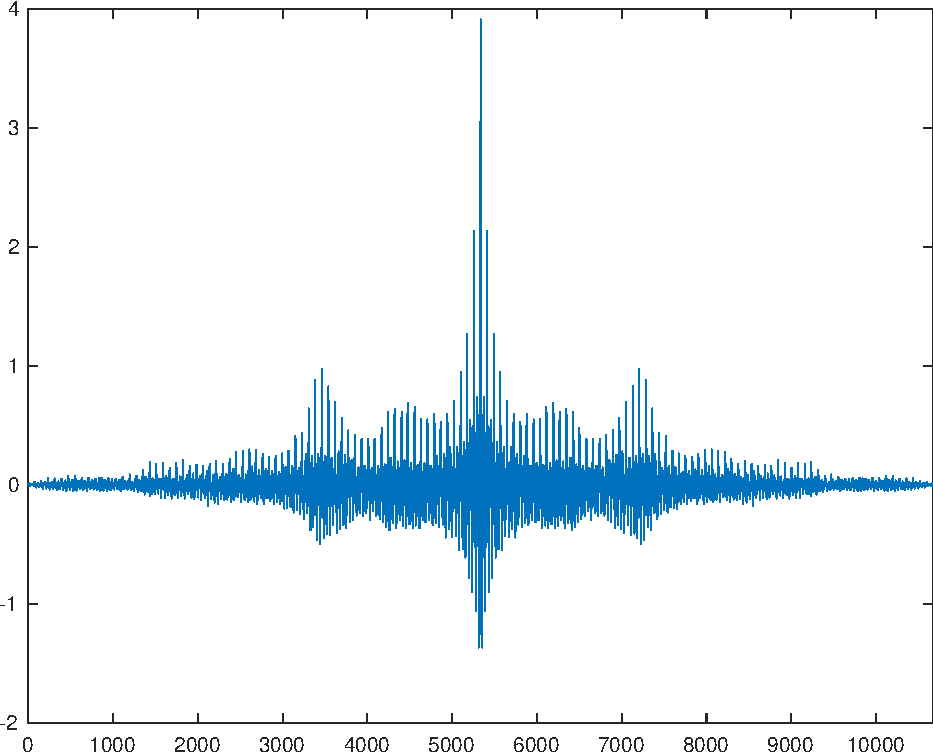
\includegraphics[width=0.8\columnwidth]{pictures/acorr_a.pdf}
    \caption{Plot of the covariance function $R_{\epsilon\epsilon}(k)$ for `a'}
    \label{fig:acorra}
\end{figure}

\begin{figure}[h!]
    \centering
    \captionsetup{justification=centering}
    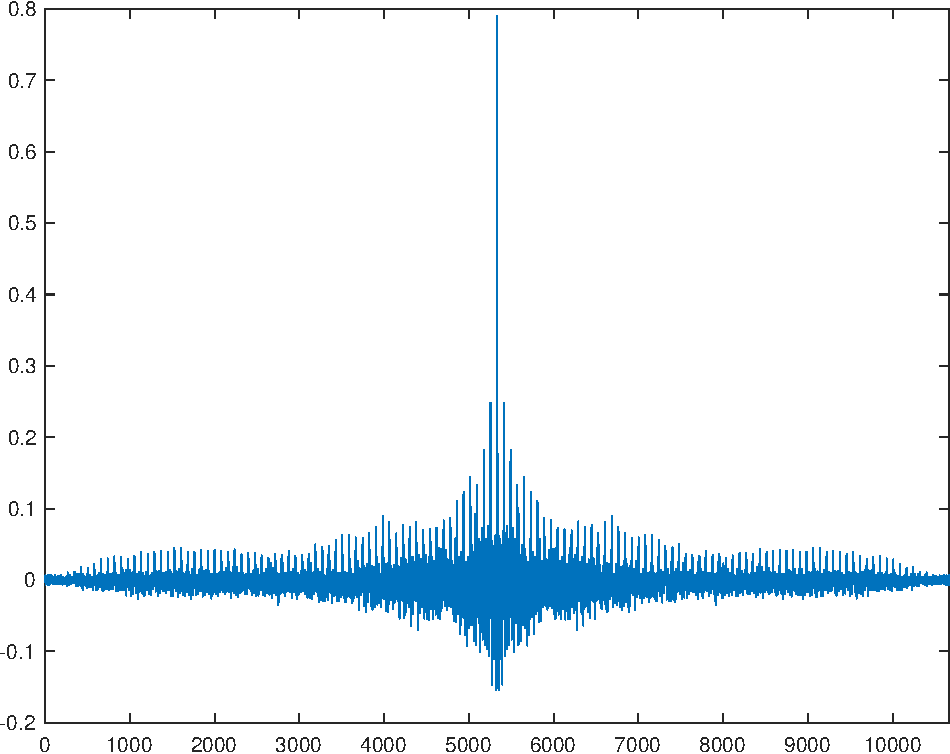
\includegraphics[width=0.8\columnwidth]{pictures/acorr_o.pdf}
    \caption{Plot of the covariance function $R_{\epsilon\epsilon}(k)$ for `o'}
    \label{fig:acorro}
\end{figure}

For the `a' vowel, the prediction comparison yielded an 86.42\% matching
between the model prediction and the validation data. This number was 92.79\%
for the `o'. The comparison plots for
the `a' and `o' models are shown in Figure \ref{fig:comparea} and Figure
\ref{fig:compareo} respectively.

\begin{figure}[h!]
    \centering
    \captionsetup{justification=centering}
    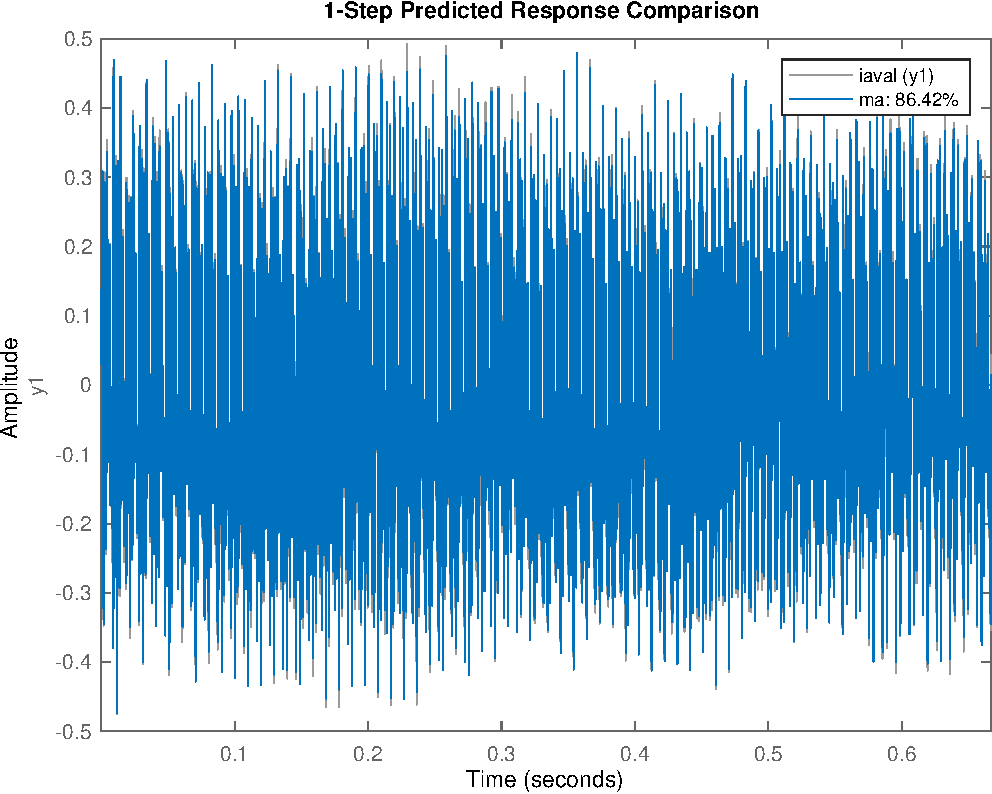
\includegraphics[width=0.8\columnwidth]{pictures/compare_a.pdf}
    \caption{Plot of the prediction comparison of the `o' model}
    \label{fig:comparea}
\end{figure}

\begin{figure}[h!]
    \centering
    \captionsetup{justification=centering}
    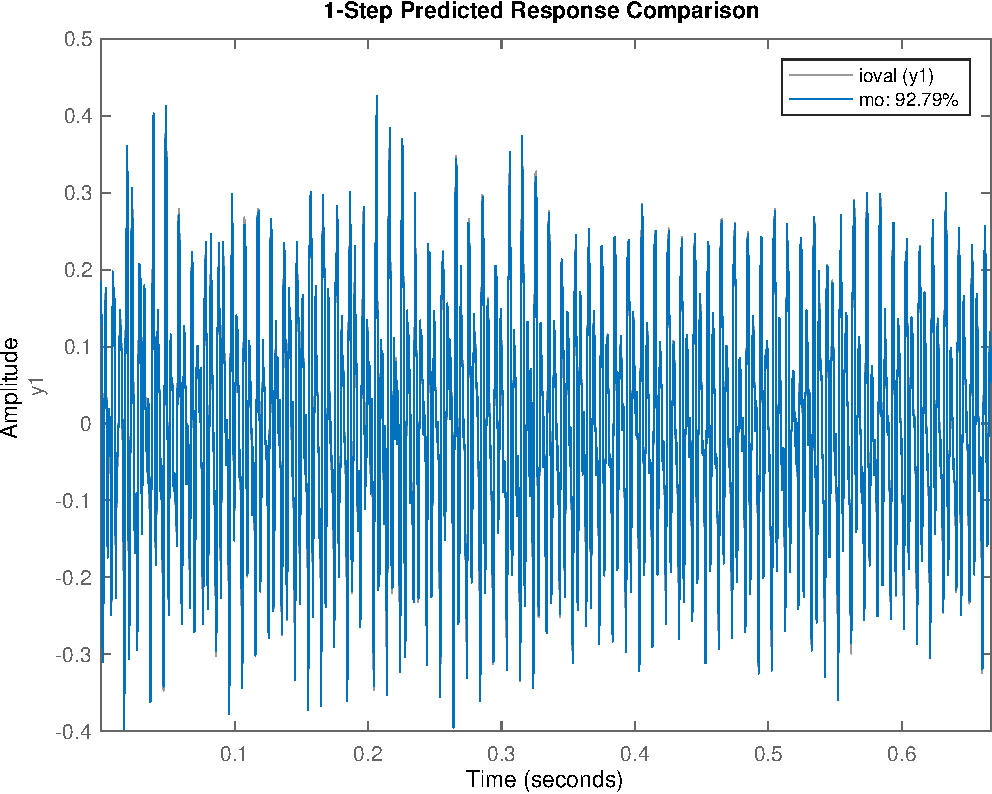
\includegraphics[width=0.8\columnwidth]{pictures/compare_o.pdf}
    \caption{Plot of the prediction comparison of the `o' model}
    \label{fig:compareo}
\end{figure}

The period of the `a' vowel was read as 78 samples, and 81 samples for the `o'
from Figure \ref{fig:rawaudio}. Using this information and the models,
simulations of the `a' and `o' vowels were created, the amplitude spectra of
which are shown in comparison to the spectra of the recorded vowels in Figure
\ref{fig:adft} and Figure \ref{fig:odft}.

\begin{figure}[h!]
    \centering
    \captionsetup{justification=centering}
    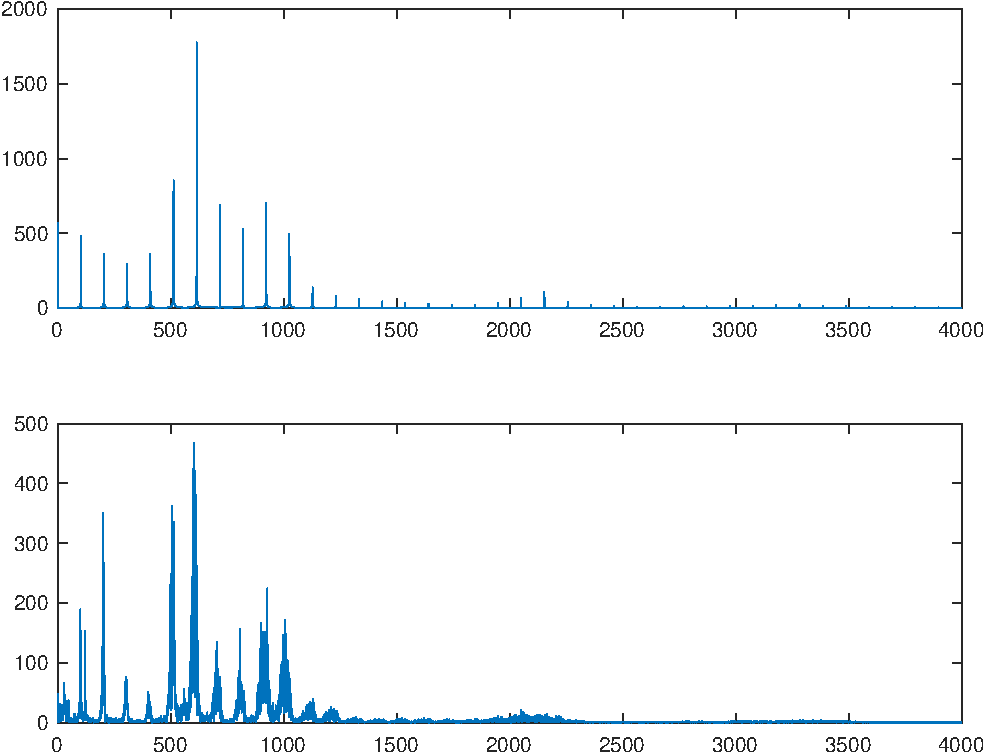
\includegraphics[width=0.8\columnwidth]{pictures/apreddft.pdf}
    \caption{Amplitude spectrum of the estimated `a' (above) and recorded
    `a' (below)}
    \label{fig:adft}
\end{figure}

\begin{figure}[h!]
    \centering
    \captionsetup{justification=centering}
    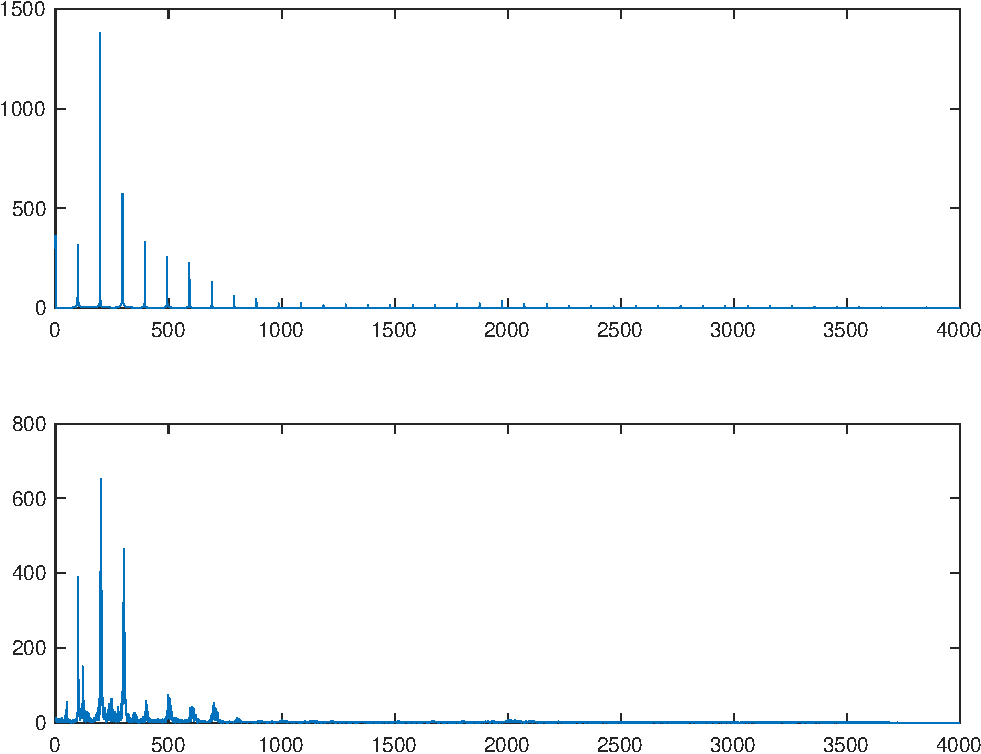
\includegraphics[width=0.8\columnwidth]{pictures/opreddft.pdf}
    \caption{Amplitude spectrum of the estimated `o' (above) and recorded
    `o' (below)}
    \label{fig:odft}
\end{figure}

The simulated vowels sounded close to the vowels they were simulating.
However, they sounded slightly synthetic, especially the `o'.

\subsection{Discussion}

The covariance functions of the residuals of the signals in Figures
\ref{fig:acorra} and \ref{fig:acorro} are small for $k \neq 0$ and
high for $k=0$, and the probability of the residuals changing sign from
one sample to the next are close to 0.5, indicating that the residuals are
approximately white. This combined with the fact that the model predictions
matched 86.42\% and 92.79\% with the validation data means that the models
were quite good. The reasons why the residuals weren't perfectly white and
the predictions didn't match 100\% is because the recordings weren't perfectly
stationary in the sense that the amplitude and pitch of the voice slightly
changed throughout the recording and that the model is only an estimate; some
information is lost.

The audio of the simulated vowels are easily identifiable as the vowels
`a' and `o', and the amplitude spectra of these in Figures \ref{fig:adft} and
\ref{fig:odft} show close resemblence to the spectra of the recorded vowels.
Since we can simulate the vowels using AR-models of orders 10 and 12, this
means we can very effectively represent these vowels using only 12 and 14
numbers (the period and amplitude of the pulse train need also be known).

Looking at the amplitude spectra of the simulated vowels compared to the
recorded ones, one can deduce that it should be possible to estimate the
suitable model order by identifying the number of large peaks in the
spectrum. Since the AR-model order corresponds to the number of poles used,
which corresponds to the number of peaks in the model's impulse response. Since
impulse trains are used as inputs to the models, there is a clear connection
between the number of peaks in the recorded signals' spectrums and the
suitable model orders to use. This means that the suitable model order
can be estimated by counting the number of significant peaks in the
recorded audio's spectrum.

\section{Assignment 3 --- GSM}

In this assignment, a simple version of the type of speech encoding used in GSM
(Global System for Mobile Communications) was to be implemented. This
implementation was then to be used to encode a short recorded sentence.

\subsection{Theory}
\label{sub:vimtheory}

The main difference between trying to model vowels and spoken language
is the amount of information that is contained within the signal.
Therefore it would be impossible to model to whole signal with a
single AR model. One approach to handle this problem is to divide
the original signal into smaller parts and then try to model each such
part individually. The overall number of parameters needed to model the
whole signal increases but this should make it possible to generate a
signal that resembles the original one. The theory for estimating a
model is similar to that for vowels in Section \ref{sub:voweltheory}.

As with vowels it is expected that spoken language is best generated
with a pulse train as input to the estimated model. Because the signal
is divided into many small parts, it is now impossible to manually choose
the amplitude and the period of the pulse train needed to generate to
signal. These can be found automatically be analyzing the autocorrelation
of the small part that is being modeled. The time delay of the first
residual peak in this function will give the approximate period of the
signal and squared root of its amplitude will be the needed amplitude of
the pulse train.

To make sure that the estimated model is not heavily biased, the signal
being modeled should be detrended before estimation. This means in this
case subtracting the mean of the signal to make sure that the
signal has $0$ mean.

When estimating a model for speech it is also possible for the poles
of the model to be outside of the unit circle, thus resulting in an
unstable system. To handle this problem we can check the poles of the
resulting model and move them inside the unit circle so that their
distance to the circle is the same as before.

Except for these small differences, the process of estimating an AR
model for the signal is done as before. The model parameters together
with the period and amplitude of the pulse train for each small part
of the signal is all that should be needed in order to generate a new
signal that resembles the original one.

\subsection{Method}
As before, the first step of this assignment was to record the audio
signal that would be analyzed and modeled. As with the other signals
this recording was done in Audacity \cite{audacity} and then cut to
the desired length. For the purpose of this assignment spoken language
was needed, so the sentence ``Vim is much easier than notepad!'' was
recorded. A graph of this recording is shown in Figure \ref{3:rawvim}.

\begin{figure}[h]
  \centering
  \captionsetup{justification=centering}

  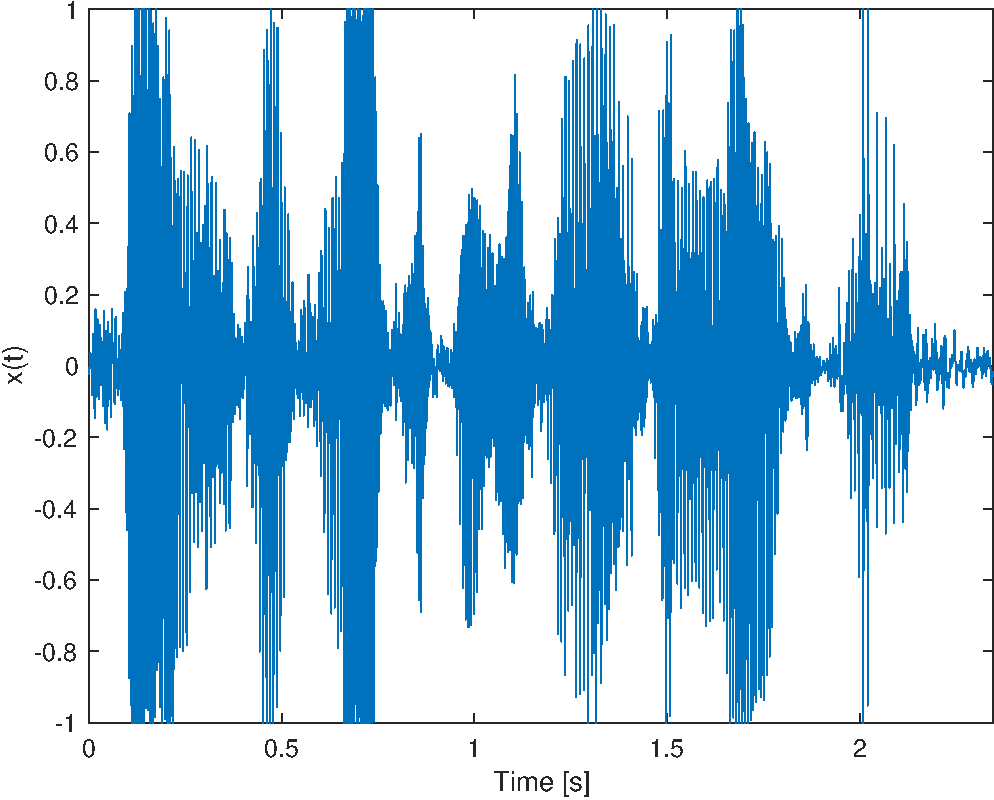
\includegraphics[width=0.8\columnwidth]{pictures/vim_orig.pdf}
  \caption{Recording of spoken language in the time domain}
  \label{3:rawvim}

\end{figure}

The first thing that was done with the recording was to split it up into
small parts of 160 samples each. Each part was then saved in a vector
of such small signal segments.

A loop was then implemented that iterated through all of the segments.
Each iteration created a model for each of the segments. All the models
and parameters needed to later recreate the signal were also saved in
vectors.

The same steps were performed on all parts each iteration. First the
signal segment was detrended. Then an AR(8) model of the segment was
estimated as before. When a model has been computed, its poles are
analyzed and moved inside the unit circle if needed. Once the poles
have been rectified, the segment was correlated with itself so that
the needed amplitude and period of the pulse train could be computed
as described in \ref{sub:vimtheory}. Because it was desired to listen
to the recreated signal, at the end of each iteration a new signal
segment was generated from each estimated model and put together into
a new whole signal. This was done by creating the needed pulse train
and inputing it into the estimated model. After the loop it was then
possible to listen to the result of modeling the signal segments with
AR(8) models. The generated audio signal is shown in Figure
\ref{3:genvim}.

\begin{figure}[h]
  \centering
  \captionsetup{justification=centering}

  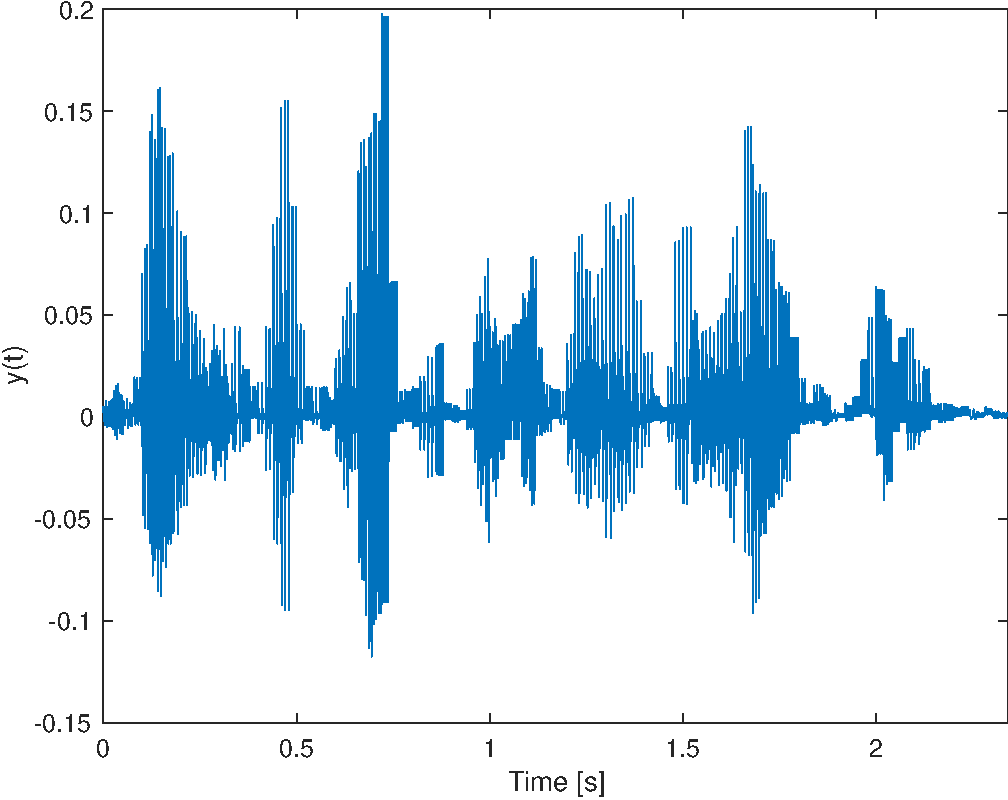
\includegraphics[width=0.8\columnwidth]{pictures/vim_gen.pdf}
  \caption{Generated audio signal of the original spoken sentence}
  \label{3:genvim}

\end{figure}

Once this was done, the whole process was repeated but the amplitude
of all the pulse trains was set to $1$ and the resulting audio signal
was played and compared to the previously generated one.

Lastly, an experiment was done to vary the model order and listen to
the result to see how the quality of the sound changed.

\subsection{Results}
The generated signal as a result of the assignment resembled the
original spoken sentence to some extent. It was possible to hear and
easily distinguish what was being said. The audio, though, was heavily
distorted and sounded very synthetic. It did not even closely resemble
the voice of the recorded person. Setting the amplitude of the pulse trains
to $1$ distorted the audio even further, to the point where it was not
even possible to hear what was being said anymore. Varying the model order
did not improve the quality of the audio much. Lowering the model order
lowered the quality of the resulting signal as expected. Increasing the
order instead did not result in any significant improvement of the
quality and in some cases the audio even sounded worse.

\subsection{Discussion}
The fact that it is hard to use the estimated models to generates the
original signal is somewhat expected because of the complexity of the
signal that is being modeled. A model described by only a few parameters
cannot confidently generate an audio signal so complex such as speech.
Also the fact that increasing the order of the estimated models did not
result in any significant increase in quality might mean that even the
type of the model used might not be appropriate for this purpose. That
the audio quality in some cases was experienced as worse when increasing
the order of the models might be beacause a lower residual error does
not necessarily mean that the signal sounds better. The experienced
quality of the sound is a subjective measure and it is hard to relate
to subtle changes in the modeling process.

Inputting pulse trains of constant amplitude $1$ into the models results
in a very distorted audio signal. This is as expected since this means
that the same ammount of energy is inputed in all of the signal segments
while the energy in the different parts of the original signal might vary
significantly. Considering these results, other methods of modeling might
be desired when modeling the sound of speech.

\section{Conclusion}

The results from this study seem to indicate that auto-regressive models are
suitable for representing simple, periodic signals, such as whistles and
vowels. It is more difficult, however, to use this technique to approximate
more complex signals, such as speech. Splitting such signals into smaller
segments might help, but the quality of the approximations might not be as
desired, and the level of compression not as high as with periodic signals.

All estimations sounded more synthetic than the recorded audio, which is to
be expected when only the "essence" of, for instance, what makes an `a' an `a'
is modeled. The natural variations in spoken vowels are discarded, since these
unpredictable variables would make the model more complicated. However, both
when modeling vowels and speech, the models were good enough to
make the information in the simulations intelligible, making this technique
suitable where only this matters.

\newpage
\begin{thebibliography}{9}

\bibitem{signalproc}
  Gustafsson, Fredrik. Ljung, Lennart. Millnert, Mille.
  \textit{Signal processing}.
  Studentlitteratur, Lund,
  2010.

\bibitem{audacity}
  Audacity \\
  \url{http://www.audacityteam.org},
  2017-11-29

\end{thebibliography}

\begin{appendices}

    \section{Matlab code}
    \subsection{sig2ar.m}\label{code:sig2ar}
    \lstinputlisting[language=Matlab]{../sig2ar.m}
    \subsection{arordercv.m}\label{code:arordercv}
    \lstinputlisting[language=Matlab]{../arordercv.m}
    \subsection{sign\_change\_prob.m}\label{code:signchangeprob}
    \lstinputlisting[language=Matlab]{../sign_change_prob.m}
    \subsection{whistle.m}\label{code:whistle}
    \lstinputlisting[language=Matlab]{../whistle.m}
    \subsection{vowels.m}\label{code:vowels}
    \lstinputlisting[language=Matlab]{../vowels.m}
    \subsection{gsm.m}\label{code:gsm}
    \lstinputlisting[language=Matlab]{../gsm.m}
\end{appendices}

\end{document}
